\documentclass[a4paper,12pt]{article}
\usepackage[margin=18mm]{geometry}
\usepackage{tikz}
\usepackage{amsmath}
\newcommand{\pFourCell}[2]{\makebox[#1em][c]{\ensuremath{#2}}}
\pagestyle{empty}
\begin{document}
\section*{Spaltentreue LaTeX-Ausgabe}
\noindent Gleichung: \texttt{sin(sqrt((x+3)/(2+1)))=5} \hfill Zielvariable: \texttt{x} \hfill Profil: \texttt{standard @3x}

\vspace{8mm}
\begin{center}
\begin{tikzpicture}[x=1em,y=-1em]
\node[anchor=base, inner sep=0pt] at (11.49,2.9) {$\pFourCell{8.82}{\sqrt{\displaystyle\frac{\pFourCell{2.7}{x}\pFourCell{2.34}{+}\pFourCell{2.64}{3}}{\pFourCell{2.7}{2}\pFourCell{2.34}{+}\pFourCell{2.64}{1}}}}$};
\node[anchor=base, inner sep=0pt] at (2.43,2.9) {$\pFourCell{4.86}{\sin}$};
\node[anchor=base, inner sep=0pt] at (5.97,2.9) {$\pFourCell{2.22}{\left(\vphantom{\pFourCell{7.68}{\sqrt{\displaystyle\frac{\pFourCell{2.7}{x}\pFourCell{2.34}{+}\pFourCell{2.64}{3}}{\pFourCell{2.7}{2}\pFourCell{2.34}{+}\pFourCell{2.64}{1}}}}}\right.}$};
\node[anchor=base, inner sep=0pt] at (17.01,2.9) {$\pFourCell{2.22}{\left.\vphantom{\pFourCell{7.68}{\sqrt{\displaystyle\frac{\pFourCell{2.7}{x}\pFourCell{2.34}{+}\pFourCell{2.64}{3}}{\pFourCell{2.7}{2}\pFourCell{2.34}{+}\pFourCell{2.64}{1}}}}}\right)}$};
\node[anchor=base, inner sep=0pt] at (20.55,2.9) {$=$};
\node[anchor=base, inner sep=0pt] at (32.88,2.9) {$5$};
\node[anchor=base, inner sep=0pt] at (11.49,7.65) {$\pFourCell{8.82}{\sqrt{\displaystyle\frac{\pFourCell{2.7}{x}\pFourCell{2.34}{+}\pFourCell{2.64}{3}}{\pFourCell{2.7}{2}\pFourCell{2.34}{+}\pFourCell{2.64}{1}}}}$};
\node[anchor=base, inner sep=0pt] at (20.55,7.65) {$=$};
\node[anchor=base, inner sep=0pt] at (32.88,7.65) {$\pFourCell{3}{5}$};
\node[anchor=base, inner sep=0pt] at (27.18,7.65) {$\pFourCell{6.12}{\arcsin}$};
\node[anchor=base, inner sep=0pt] at (30.81,7.65) {$\pFourCell{1.14}{\left(\vphantom{\pFourCell{3}{5}}\right.}$};
\node[anchor=base, inner sep=0pt] at (34.95,7.65) {$\pFourCell{1.14}{\left.\vphantom{\pFourCell{3}{5}}\right)}$};
\node[anchor=base, inner sep=0pt] at (12.06,12.075) {$\displaystyle\frac{\pFourCell{2.7}{x}\pFourCell{2.34}{+}\pFourCell{2.64}{3}}{\pFourCell{2.7}{2}\pFourCell{2.34}{+}\pFourCell{2.64}{1}}$};
\node[anchor=base, inner sep=0pt] at (20.55,12.075) {$=$};
\node[anchor=base, inner sep=0pt] at (32.88,12.075) {$\pFourCell{3}{5}$};
\node[anchor=base, inner sep=0pt] at (23.55,12.075) {$\pFourCell{1.14}{\left(\vphantom{\pFourCell{3}{\arcsin\left(5\right)}}\right.}$};
\node[anchor=base, inner sep=0pt] at (37.59,12.075) {$\pFourCell{4.14}{\left.\vphantom{\pFourCell{3}{\arcsin\left(5\right)}}\right)^{2}}$};
\node[anchor=base, inner sep=0pt] at (27.18,12.075) {$\pFourCell{6.12}{\arcsin}$};
\node[anchor=base, inner sep=0pt] at (30.81,12.075) {$\pFourCell{1.14}{\left(\vphantom{\pFourCell{3}{5}}\right.}$};
\node[anchor=base, inner sep=0pt] at (34.95,12.075) {$\pFourCell{1.14}{\left.\vphantom{\pFourCell{3}{5}}\right)}$};
\node[anchor=base, inner sep=0pt] at (9.57,15.535) {$x$};
\node[anchor=base, inner sep=0pt] at (12.09,15.535) {$+$};
\node[anchor=base, inner sep=0pt] at (14.58,15.535) {$3$};
\node[anchor=base, inner sep=0pt] at (20.55,15.535) {$=$};
\node[anchor=base, inner sep=0pt] at (32.88,15.535) {$\pFourCell{3}{5}$};
\node[anchor=base, inner sep=0pt] at (23.55,15.535) {$\pFourCell{1.14}{\left(\vphantom{\pFourCell{3}{\arcsin\left(5\right)}}\right.}$};
\node[anchor=base, inner sep=0pt] at (37.59,15.535) {$\pFourCell{4.14}{\left.\vphantom{\pFourCell{3}{\arcsin\left(5\right)}}\right)^{2}}$};
\node[anchor=base, inner sep=0pt] at (27.18,15.535) {$\pFourCell{6.12}{\arcsin}$};
\node[anchor=base, inner sep=0pt] at (30.81,15.535) {$\pFourCell{1.14}{\left(\vphantom{\pFourCell{3}{5}}\right.}$};
\node[anchor=base, inner sep=0pt] at (34.95,15.535) {$\pFourCell{1.14}{\left.\vphantom{\pFourCell{3}{5}}\right)}$};
\node[anchor=base, inner sep=0pt] at (44.79,15.535) {$\pFourCell{3}{2}\pFourCell{2.34}{+}\pFourCell{2.64}{1}$};
\node[anchor=base, inner sep=0pt] at (40.23,15.535) {$\pFourCell{1.14}{\left(\vphantom{\pFourCell{3}{2}\pFourCell{2.34}{+}\pFourCell{2.64}{1}}\right.}$};
\node[anchor=base, inner sep=0pt] at (49.35,15.535) {$\pFourCell{1.14}{\left.\vphantom{\pFourCell{3}{2}\pFourCell{2.34}{+}\pFourCell{2.64}{1}}\right)}$};
\node[anchor=base, inner sep=0pt] at (9.57,18.355) {$x$};
\node[anchor=base, inner sep=0pt] at (20.55,18.355) {$=$};
\node[anchor=base, inner sep=0pt] at (32.88,18.355) {$\pFourCell{3}{5}$};
\node[anchor=base, inner sep=0pt] at (23.55,18.355) {$\pFourCell{1.14}{\left(\vphantom{\pFourCell{3}{\arcsin\left(5\right)}}\right.}$};
\node[anchor=base, inner sep=0pt] at (37.59,18.355) {$\pFourCell{4.14}{\left.\vphantom{\pFourCell{3}{\arcsin\left(5\right)}}\right)^{2}}$};
\node[anchor=base, inner sep=0pt] at (27.18,18.355) {$\pFourCell{6.12}{\arcsin}$};
\node[anchor=base, inner sep=0pt] at (30.81,18.355) {$\pFourCell{1.14}{\left(\vphantom{\pFourCell{3}{5}}\right.}$};
\node[anchor=base, inner sep=0pt] at (34.95,18.355) {$\pFourCell{1.14}{\left.\vphantom{\pFourCell{3}{5}}\right)}$};
\node[anchor=base, inner sep=0pt] at (44.79,18.355) {$\pFourCell{3}{2}\pFourCell{2.34}{+}\pFourCell{2.64}{1}$};
\node[anchor=base, inner sep=0pt] at (40.23,18.355) {$\pFourCell{1.14}{\left(\vphantom{\pFourCell{3}{2}\pFourCell{2.34}{+}\pFourCell{2.64}{1}}\right.}$};
\node[anchor=base, inner sep=0pt] at (49.35,18.355) {$\pFourCell{1.14}{\left.\vphantom{\pFourCell{3}{2}\pFourCell{2.34}{+}\pFourCell{2.64}{1}}\right)}$};
\node[anchor=base, inner sep=0pt] at (51.09,18.355) {$-$};
\node[anchor=base, inner sep=0pt] at (53.58,18.355) {$3$};
\end{tikzpicture}
\end{center}

\newpage
\section*{Spaltentreue LaTeX-Ausgabe mit Spaltengrenzen}
\vspace{6mm}
\begin{center}
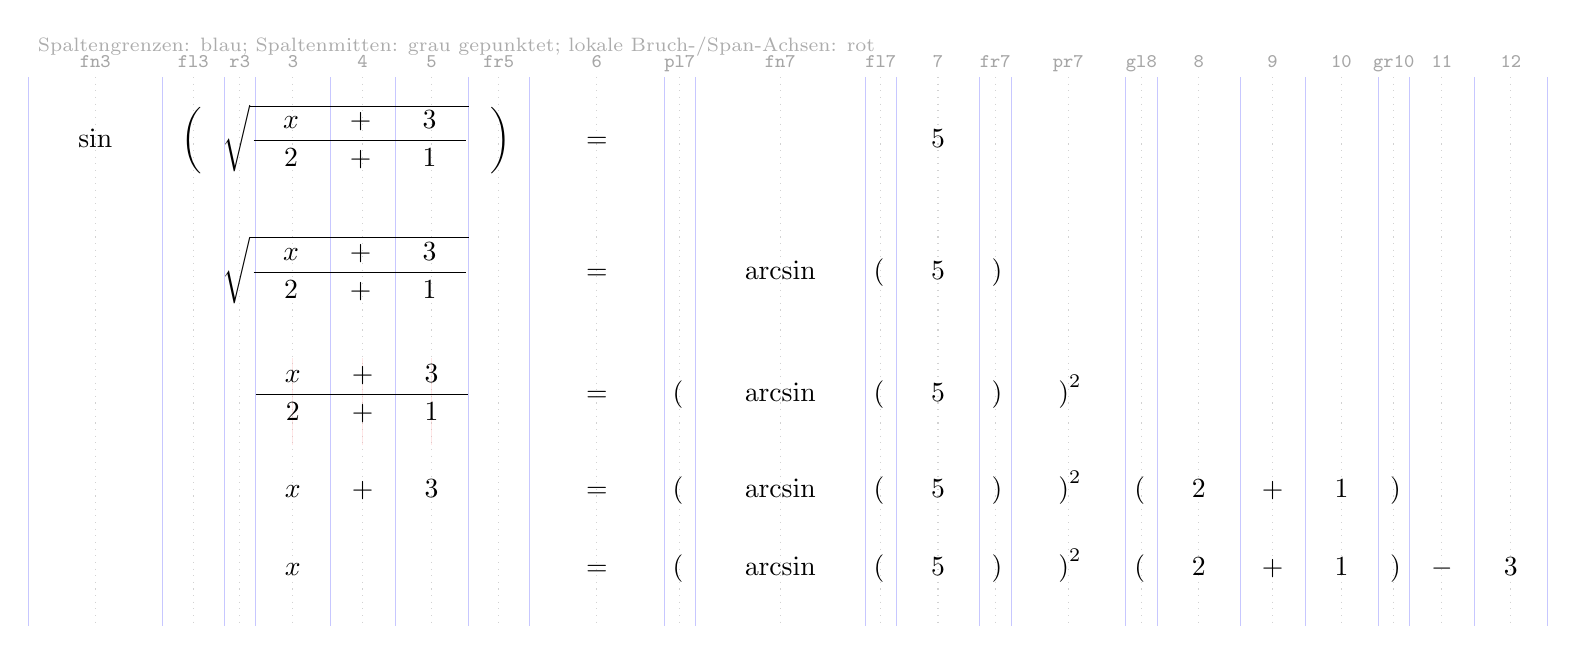
\begin{tikzpicture}[x=1em,y=-1em]
\node[font={\scriptsize}, text=gray!65, anchor=west] at (0,-0.75) {Spaltengrenzen: blau; Spaltenmitten: grau gepunktet; lokale Bruch-/Span-Achsen: rot};
\draw[blue!22, line width=0.28pt] (0,0.35) -- (0,20.19);
\draw[blue!22, line width=0.28pt] (4.86,0.35) -- (4.86,20.19);
\draw[blue!22, line width=0.28pt] (7.08,0.35) -- (7.08,20.19);
\draw[blue!22, line width=0.28pt] (8.22,0.35) -- (8.22,20.19);
\draw[blue!22, line width=0.28pt] (10.92,0.35) -- (10.92,20.19);
\draw[blue!22, line width=0.28pt] (13.26,0.35) -- (13.26,20.19);
\draw[blue!22, line width=0.28pt] (15.9,0.35) -- (15.9,20.19);
\draw[blue!22, line width=0.28pt] (18.12,0.35) -- (18.12,20.19);
\draw[blue!22, line width=0.28pt] (22.98,0.35) -- (22.98,20.19);
\draw[blue!22, line width=0.28pt] (24.12,0.35) -- (24.12,20.19);
\draw[blue!22, line width=0.28pt] (30.24,0.35) -- (30.24,20.19);
\draw[blue!22, line width=0.28pt] (31.38,0.35) -- (31.38,20.19);
\draw[blue!22, line width=0.28pt] (34.38,0.35) -- (34.38,20.19);
\draw[blue!22, line width=0.28pt] (35.52,0.35) -- (35.52,20.19);
\draw[blue!22, line width=0.28pt] (39.66,0.35) -- (39.66,20.19);
\draw[blue!22, line width=0.28pt] (40.8,0.35) -- (40.8,20.19);
\draw[blue!22, line width=0.28pt] (43.8,0.35) -- (43.8,20.19);
\draw[blue!22, line width=0.28pt] (46.14,0.35) -- (46.14,20.19);
\draw[blue!22, line width=0.28pt] (48.78,0.35) -- (48.78,20.19);
\draw[blue!22, line width=0.28pt] (49.92,0.35) -- (49.92,20.19);
\draw[blue!22, line width=0.28pt] (52.26,0.35) -- (52.26,20.19);
\draw[blue!22, line width=0.28pt] (54.9,0.35) -- (54.9,20.19);
\draw[gray!35, dotted] (2.43,0.35) -- (2.43,20.19);
\node[font={\ttfamily\scriptsize}, text=gray!70, anchor=base] at (2.43,0) {fn3};
\draw[gray!35, dotted] (5.97,0.35) -- (5.97,20.19);
\node[font={\ttfamily\scriptsize}, text=gray!70, anchor=base] at (5.97,0) {fl3};
\draw[gray!35, dotted] (7.65,0.35) -- (7.65,20.19);
\node[font={\ttfamily\scriptsize}, text=gray!70, anchor=base] at (7.65,0) {r3};
\draw[gray!35, dotted] (9.57,0.35) -- (9.57,20.19);
\node[font={\ttfamily\scriptsize}, text=gray!70, anchor=base] at (9.57,0) {3};
\draw[gray!35, dotted] (12.09,0.35) -- (12.09,20.19);
\node[font={\ttfamily\scriptsize}, text=gray!70, anchor=base] at (12.09,0) {4};
\draw[gray!35, dotted] (14.58,0.35) -- (14.58,20.19);
\node[font={\ttfamily\scriptsize}, text=gray!70, anchor=base] at (14.58,0) {5};
\draw[gray!35, dotted] (17.01,0.35) -- (17.01,20.19);
\node[font={\ttfamily\scriptsize}, text=gray!70, anchor=base] at (17.01,0) {fr5};
\draw[gray!35, dotted] (20.55,0.35) -- (20.55,20.19);
\node[font={\ttfamily\scriptsize}, text=gray!70, anchor=base] at (20.55,0) {6};
\draw[gray!35, dotted] (23.55,0.35) -- (23.55,20.19);
\node[font={\ttfamily\scriptsize}, text=gray!70, anchor=base] at (23.55,0) {pl7};
\draw[gray!35, dotted] (27.18,0.35) -- (27.18,20.19);
\node[font={\ttfamily\scriptsize}, text=gray!70, anchor=base] at (27.18,0) {fn7};
\draw[gray!35, dotted] (30.81,0.35) -- (30.81,20.19);
\node[font={\ttfamily\scriptsize}, text=gray!70, anchor=base] at (30.81,0) {fl7};
\draw[gray!35, dotted] (32.88,0.35) -- (32.88,20.19);
\node[font={\ttfamily\scriptsize}, text=gray!70, anchor=base] at (32.88,0) {7};
\draw[gray!35, dotted] (34.95,0.35) -- (34.95,20.19);
\node[font={\ttfamily\scriptsize}, text=gray!70, anchor=base] at (34.95,0) {fr7};
\draw[gray!35, dotted] (37.59,0.35) -- (37.59,20.19);
\node[font={\ttfamily\scriptsize}, text=gray!70, anchor=base] at (37.59,0) {pr7};
\draw[gray!35, dotted] (40.23,0.35) -- (40.23,20.19);
\node[font={\ttfamily\scriptsize}, text=gray!70, anchor=base] at (40.23,0) {gl8};
\draw[gray!35, dotted] (42.3,0.35) -- (42.3,20.19);
\node[font={\ttfamily\scriptsize}, text=gray!70, anchor=base] at (42.3,0) {8};
\draw[gray!35, dotted] (44.97,0.35) -- (44.97,20.19);
\node[font={\ttfamily\scriptsize}, text=gray!70, anchor=base] at (44.97,0) {9};
\draw[gray!35, dotted] (47.46,0.35) -- (47.46,20.19);
\node[font={\ttfamily\scriptsize}, text=gray!70, anchor=base] at (47.46,0) {10};
\draw[gray!35, dotted] (49.35,0.35) -- (49.35,20.19);
\node[font={\ttfamily\scriptsize}, text=gray!70, anchor=base] at (49.35,0) {gr10};
\draw[gray!35, dotted] (51.09,0.35) -- (51.09,20.19);
\node[font={\ttfamily\scriptsize}, text=gray!70, anchor=base] at (51.09,0) {11};
\draw[gray!35, dotted] (53.58,0.35) -- (53.58,20.19);
\node[font={\ttfamily\scriptsize}, text=gray!70, anchor=base] at (53.58,0) {12};
\node[anchor=base, inner sep=0pt] at (11.49,2.9) {$\pFourCell{8.82}{\sqrt{\displaystyle\frac{\pFourCell{2.7}{x}\pFourCell{2.34}{+}\pFourCell{2.64}{3}}{\pFourCell{2.7}{2}\pFourCell{2.34}{+}\pFourCell{2.64}{1}}}}$};
\node[anchor=base, inner sep=0pt] at (2.43,2.9) {$\pFourCell{4.86}{\sin}$};
\node[anchor=base, inner sep=0pt] at (5.97,2.9) {$\pFourCell{2.22}{\left(\vphantom{\pFourCell{7.68}{\sqrt{\displaystyle\frac{\pFourCell{2.7}{x}\pFourCell{2.34}{+}\pFourCell{2.64}{3}}{\pFourCell{2.7}{2}\pFourCell{2.34}{+}\pFourCell{2.64}{1}}}}}\right.}$};
\node[anchor=base, inner sep=0pt] at (17.01,2.9) {$\pFourCell{2.22}{\left.\vphantom{\pFourCell{7.68}{\sqrt{\displaystyle\frac{\pFourCell{2.7}{x}\pFourCell{2.34}{+}\pFourCell{2.64}{3}}{\pFourCell{2.7}{2}\pFourCell{2.34}{+}\pFourCell{2.64}{1}}}}}\right)}$};
\node[anchor=base, inner sep=0pt] at (20.55,2.9) {$=$};
\node[anchor=base, inner sep=0pt] at (32.88,2.9) {$5$};
\node[anchor=base, inner sep=0pt] at (11.49,7.65) {$\pFourCell{8.82}{\sqrt{\displaystyle\frac{\pFourCell{2.7}{x}\pFourCell{2.34}{+}\pFourCell{2.64}{3}}{\pFourCell{2.7}{2}\pFourCell{2.34}{+}\pFourCell{2.64}{1}}}}$};
\node[anchor=base, inner sep=0pt] at (20.55,7.65) {$=$};
\node[anchor=base, inner sep=0pt] at (32.88,7.65) {$\pFourCell{3}{5}$};
\node[anchor=base, inner sep=0pt] at (27.18,7.65) {$\pFourCell{6.12}{\arcsin}$};
\node[anchor=base, inner sep=0pt] at (30.81,7.65) {$\pFourCell{1.14}{\left(\vphantom{\pFourCell{3}{5}}\right.}$};
\node[anchor=base, inner sep=0pt] at (34.95,7.65) {$\pFourCell{1.14}{\left.\vphantom{\pFourCell{3}{5}}\right)}$};
\draw[red!30, opacity=0.32, line width=0.35pt] (9.57,10.5) -- (9.57,13.65);
\draw[red!30, opacity=0.32, line width=0.35pt] (12.09,10.5) -- (12.09,13.65);
\draw[red!30, opacity=0.32, line width=0.35pt] (14.58,10.5) -- (14.58,13.65);
\node[anchor=base, inner sep=0pt] at (12.06,12.075) {$\displaystyle\frac{\pFourCell{2.7}{x}\pFourCell{2.34}{+}\pFourCell{2.64}{3}}{\pFourCell{2.7}{2}\pFourCell{2.34}{+}\pFourCell{2.64}{1}}$};
\node[anchor=base, inner sep=0pt] at (20.55,12.075) {$=$};
\node[anchor=base, inner sep=0pt] at (32.88,12.075) {$\pFourCell{3}{5}$};
\node[anchor=base, inner sep=0pt] at (23.55,12.075) {$\pFourCell{1.14}{\left(\vphantom{\pFourCell{3}{\arcsin\left(5\right)}}\right.}$};
\node[anchor=base, inner sep=0pt] at (37.59,12.075) {$\pFourCell{4.14}{\left.\vphantom{\pFourCell{3}{\arcsin\left(5\right)}}\right)^{2}}$};
\node[anchor=base, inner sep=0pt] at (27.18,12.075) {$\pFourCell{6.12}{\arcsin}$};
\node[anchor=base, inner sep=0pt] at (30.81,12.075) {$\pFourCell{1.14}{\left(\vphantom{\pFourCell{3}{5}}\right.}$};
\node[anchor=base, inner sep=0pt] at (34.95,12.075) {$\pFourCell{1.14}{\left.\vphantom{\pFourCell{3}{5}}\right)}$};
\node[anchor=base, inner sep=0pt] at (9.57,15.535) {$x$};
\node[anchor=base, inner sep=0pt] at (12.09,15.535) {$+$};
\node[anchor=base, inner sep=0pt] at (14.58,15.535) {$3$};
\node[anchor=base, inner sep=0pt] at (20.55,15.535) {$=$};
\node[anchor=base, inner sep=0pt] at (32.88,15.535) {$\pFourCell{3}{5}$};
\node[anchor=base, inner sep=0pt] at (23.55,15.535) {$\pFourCell{1.14}{\left(\vphantom{\pFourCell{3}{\arcsin\left(5\right)}}\right.}$};
\node[anchor=base, inner sep=0pt] at (37.59,15.535) {$\pFourCell{4.14}{\left.\vphantom{\pFourCell{3}{\arcsin\left(5\right)}}\right)^{2}}$};
\node[anchor=base, inner sep=0pt] at (27.18,15.535) {$\pFourCell{6.12}{\arcsin}$};
\node[anchor=base, inner sep=0pt] at (30.81,15.535) {$\pFourCell{1.14}{\left(\vphantom{\pFourCell{3}{5}}\right.}$};
\node[anchor=base, inner sep=0pt] at (34.95,15.535) {$\pFourCell{1.14}{\left.\vphantom{\pFourCell{3}{5}}\right)}$};
\node[anchor=base, inner sep=0pt] at (44.79,15.535) {$\pFourCell{3}{2}\pFourCell{2.34}{+}\pFourCell{2.64}{1}$};
\node[anchor=base, inner sep=0pt] at (40.23,15.535) {$\pFourCell{1.14}{\left(\vphantom{\pFourCell{3}{2}\pFourCell{2.34}{+}\pFourCell{2.64}{1}}\right.}$};
\node[anchor=base, inner sep=0pt] at (49.35,15.535) {$\pFourCell{1.14}{\left.\vphantom{\pFourCell{3}{2}\pFourCell{2.34}{+}\pFourCell{2.64}{1}}\right)}$};
\node[anchor=base, inner sep=0pt] at (9.57,18.355) {$x$};
\node[anchor=base, inner sep=0pt] at (20.55,18.355) {$=$};
\node[anchor=base, inner sep=0pt] at (32.88,18.355) {$\pFourCell{3}{5}$};
\node[anchor=base, inner sep=0pt] at (23.55,18.355) {$\pFourCell{1.14}{\left(\vphantom{\pFourCell{3}{\arcsin\left(5\right)}}\right.}$};
\node[anchor=base, inner sep=0pt] at (37.59,18.355) {$\pFourCell{4.14}{\left.\vphantom{\pFourCell{3}{\arcsin\left(5\right)}}\right)^{2}}$};
\node[anchor=base, inner sep=0pt] at (27.18,18.355) {$\pFourCell{6.12}{\arcsin}$};
\node[anchor=base, inner sep=0pt] at (30.81,18.355) {$\pFourCell{1.14}{\left(\vphantom{\pFourCell{3}{5}}\right.}$};
\node[anchor=base, inner sep=0pt] at (34.95,18.355) {$\pFourCell{1.14}{\left.\vphantom{\pFourCell{3}{5}}\right)}$};
\node[anchor=base, inner sep=0pt] at (44.79,18.355) {$\pFourCell{3}{2}\pFourCell{2.34}{+}\pFourCell{2.64}{1}$};
\node[anchor=base, inner sep=0pt] at (40.23,18.355) {$\pFourCell{1.14}{\left(\vphantom{\pFourCell{3}{2}\pFourCell{2.34}{+}\pFourCell{2.64}{1}}\right.}$};
\node[anchor=base, inner sep=0pt] at (49.35,18.355) {$\pFourCell{1.14}{\left.\vphantom{\pFourCell{3}{2}\pFourCell{2.34}{+}\pFourCell{2.64}{1}}\right)}$};
\node[anchor=base, inner sep=0pt] at (51.09,18.355) {$-$};
\node[anchor=base, inner sep=0pt] at (53.58,18.355) {$3$};
\end{tikzpicture}
\end{center}
\end{document}
